\documentclass[a4paper,norsk,11pt]{article}
\usepackage[utf8x]{inputenc}
\usepackage{babel}
%\usepackage[firstpage]{draftwatermark}
\usepackage{graphicx}
\usepackage{geometry} 
\usepackage[hyphens]{url}
\usepackage{hyperref}

%opening
\title{Bruksanvisning for Sonja}
\author{Knut Hegna}
%\SetWatermarkColor{red}
%\SetWatermarkText{Dette dokumentet er under arbeid!}
%\SetWatermarkLightness{0.7}
\begin{document}

\maketitle
\tableofcontents
\section{Innledning}
Programmet ligger på 

\verb=\\app-evs\w3-vh\no.uio.www_80\ub\emnesok\program\sonja\Sonja.jar= 

\noindent{}Lag en snarvei dit og legg snarveien på skrivebordet. Da er du sikret siste (og riktige) versjon. 

Programmet fungerer bare under Windows og da med følgende definisjoner av disker:

\begin{center}
 \begin{tabular}{|l|l|}\hline
  Z:&\verb=\\app-evs\w3-vh\no.uio.www_80\ub\emnesok\htdocs\data=\\\hline
  U:&\verb=\\kant\ub-ureal\felles=\\\hline
 \end{tabular}
\end{center}

\noindent{}Programmet legger oppdaterte data  på Z:-disken der de er tilgjengelige for Roald-brukere, for RDF/SQL-brukere og for Web-søket. Mer om det i avsnitt~\ref{eksport} på side~\pageref{eksport}.
\section{Testing, trening og opplæring}
Lag deg én eller flere testtermer som du tester med. La testtermene begynne med en fast tekst, så de blir lette å finne tilbake til. Så kan du legge til og fjerne data på termene, lage relasjoner osv.
\begin{enumerate}
\item Test gjerne at programmet gjør det som bruksanvisningen påstår blir gjort.
\item Sjekk at programmet har oppførsel som stemmer overens med dine forventninger.
\item Forsøk å gjøre endringer/rettelser som du mener er feil og som du forventer at programmet skal reagere på
\item Gjør endringer i originale data og lagre dem. Start programmet på nytt med oppdaterte data og sjekk at rettelser og tilføyelser er med.
\end{enumerate}
Finner du feil, så forsøk å gjenta prosedyren og gi beskjed.

\section{Søking og trefflisteklikk}
Når dataene er initiert, kan du søke på samme vis som i Roald. Søking er venstre- og høyretrunkert, men dette kan du regulere med likhetstegn.
\begin{description}
\item[Ett venstreklikk i trefflista] Markerer et treff og viser detaljer om termen eller strengen i skjemaform og du kan rette i feltene.
\item[Ett høyreklikk i trefflista] Setter inn valgt term som se også-term til den termen som er valgt med vanlig klikk (gjelder termer)
\item[Ett Ctrl-klikk i trefflista] Setter inn valgt term i det feltet du holder på å bygge i en streng.
\end{description}
\section{Behandling av indekstermer}
Se figur~\ref{termskjema}.

\begin{figure}
\begin{center}
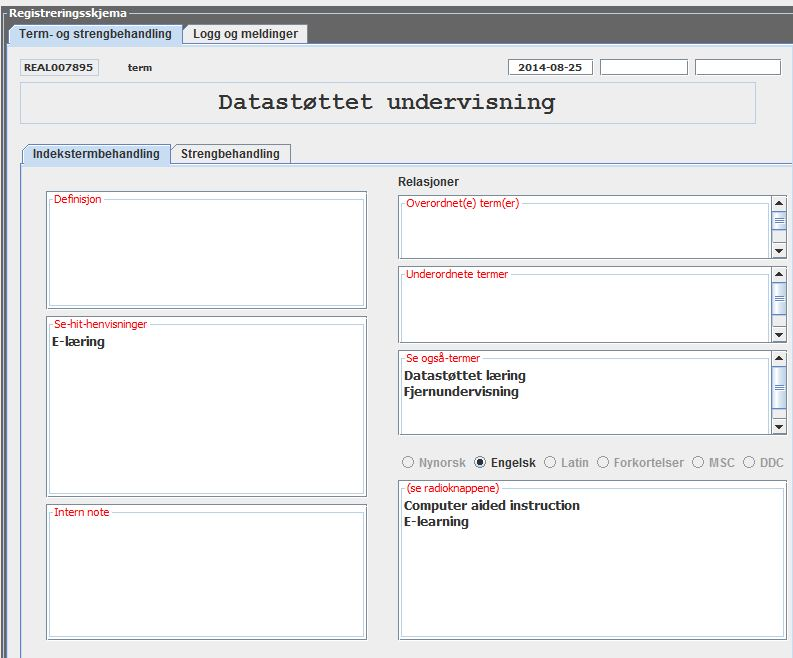
\includegraphics[width=\textwidth]{./termskjema.JPG}
\caption{Skjema for behandling av termer}\label{termskjema}
\end{center}
\end{figure}
I feltene \textit{Definisjon} og \textit{Intern note} er det nok å venstreklikke i feltet for å gjøre endringer. I de øvrige feltene er det nok å venstreklikke for å legge til nytt element. Høyreklikking gir mulighet for å slette og endre rekkefølge der det er aktuelt.

Feltene for overordnet og underordnete termer: det blir ikke foretatt omfattende konsistens-sjekker på hierarkibruken. Det blir gjort av skosify på xml-filen.

Feltet nederst til venstre (se figur~\ref{nynorskmm}) viser informasjon avhengig av hvilken radioknapp som er valgt. Bare radioknapper der det fins underliggende informasjon er aktive. Du kan venstreklikke for å legge til noe i den synlige informasjon. Du kan høyreklikke for å legge til, fjerne eller endre rekkefølge i aktive og inaktive felt.

\begin{figure}
\begin{center}
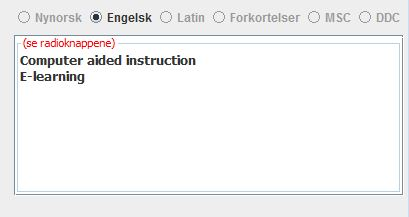
\includegraphics[width=8cm]{./nynorskmm.JPG}
\caption{Fellesfelt for nynorsk, engelsk, latin, forkortelser, dewey og MSC}\label{nynorskmm}
\end{center}
\end{figure}

\section{Behandling av strenger}
Se figur~\ref{strengskjema}.
\begin{figure}
\begin{center}
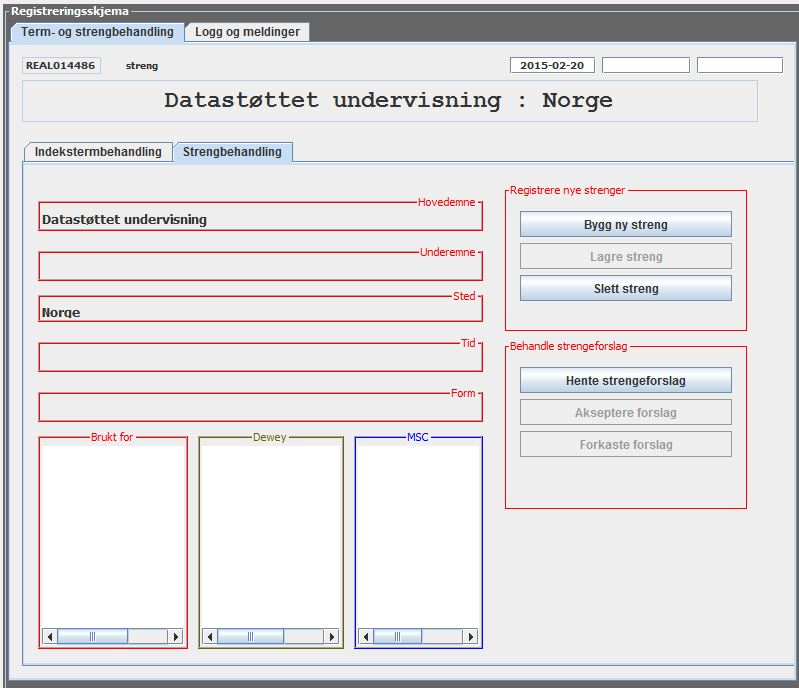
\includegraphics[width=\textwidth]{./strengskjema.JPG}
\caption{Skjema for behandling av strenger}\label{strengskjema}
\end{center}
\end{figure}

\begin{description}
\item[Endre eksisterende streng] den eneste endringen man kan gjøre er ekstrafeletene \textit{Brukt for}, \textit{Dewey} og \textit{MSC}. Bygg heller en ny streng og slett den gamle.
\item[Slett streng] Aktuelt når man har markert en streng i en treffliste.
\item[Brukt for, Dewey og MSC] Klikk i aktuelt felt for å legge til opplysning. Høyreklikk for å fjerne.
\item[Bygg ny streng] Det enkleste er å bruke Roald for å legge nye strenger i forslagskassa, som så kan behandles her. \textbf{Men}: Knappen endrer navn til \textit{Lagre ny streng} og du kan begynne å klikke i feltene for å legge inn data. Dersom betegnelsen du oppgir bare har ett treff i termtypen, blir den lagt inn automatisk. I motsatt fall får du en treffliste de kan CTRL-klikke i for å velge. Lagre strengen ved å klikke på Lagre-knappen. Programmet sjekker om strengen fins fra før. 

Sjekk at strengen er kommet inn i datagrunnlaget ved å søke på den.
\item[Strengeforslag] Forslag ligger i to filer som begge kan være tomme. Disse filene:\newline
{\footnotesize
\url{U:/Prosjekt687/roald2/data/forslagskasse.txt}\newline
\url{U:/Prosjekt687/roald2/data/arbeidskasse.txt}\newline}
Når man klikker på knappen, flyttes eventuelle data fra forslagskassa over til arbeidskassa og så arbeider man videre på den. En markert term kan aksepteres og får da identifikator. Forslaget kan også slettes og fjernes da fra arbeidskassa.

Det slo meg at programmet ikke sjekker at de enkelte delene av strengen ikke er endret siden forslaget ble sendt inn. Foreløpig må dette gjøres av redaksjonsmedlemmet.

\end{description}

\section{Omveier-menyen}
\begin{description}
\item[Registrere ny term] (Alt-N) Skriv inn betegnelsen og velg termtype. Dersom du samtidig planlegger  å legge inn se-henvisninger (synonymer), sjekk først om disse allerede ligger inne som foretrukken term. Da er det bedre å arbeide ut fra en av dem, så slipper man å generere ny id.
\item[Bytte BF og term] Viss det er mer enn én BF, kommer det opp en meny som du kan velge fra. \textit{Dette genererer data til bruk i lokar/sjanr-skjermen i BIBSYS}.
\item[Slå sammen to termer] Oppgi først den som skal bli stående, deretter den som skal slås inn under første term. Den termen som skal fjernes, blir erstattet av den som blir stående, f.eks i strenger og SO-relasjoner. \textit{Dette genererer data til bruk i lokar/sjanr-skjermen i BIBSYS}.
\item[Fjerne term] Se også-relasjoner til/fra denne termen blir fjernet. Medfører også at alle strenger som inneholder termen blir fjernet. \textit{ Dette genererer data til bruk i lokar/sjanr-skjermen i BIBSYS}.
\item[Legge til MSC] Klikk like gjerne i MSC-feltet.
\item[Legge til DDC]  Klikk like gjerne i DDC-feltet.
\item[Revidere definisjon] Klikk like gjerne i definisjonsfeltet.
\item[Revidere intern note] Klikk like gjerne i notefeltet.
\item[Vis endringsloggen] Viser endringsloggen under fanen \textit{Logg og meldinger}. Det som måttes stå der fra før slettes bortsett fra oppstartsstatus.
\end{description}

\section{Annen funksjonalitet}
\begin{description}
\item[Legge til betegnelse i et felt] Generelt: Klikk i det feltet du ønsker å legge til en ny betegnelse. Det blir gjennomført en del kontroller for å sikre konsistens i vokabularet. Blir det konflikt, vil programmet legge til rette for eksakt søk i den formtypen der konflikten opptrer.
\item[Legge til se også-term] Du kan skrive inn en helt ny term og den vil da bli opprettet som indeksterm med samme termtype. Skriver du noe som gir ett treff i datagrunnlaget antar programmet at det er termen som skal ha relasjonen. Er det flere treff på det du skriver inn, får du en vanlig treffliste. Bruk Ctrl-klikk for å velge se også-term.

Når akseptabel term er valgt, blir du spurt om det skal opprettes invers se også-relasjon.
\item[Fjerne betegnelse fra felt] Høyreklikk i feltet og velg fra oppsprettsmeny. Er det bare én i feltet, blir den fjernet. Forøvrig må du velge i en oppsprettsmeny.
\item[Bestemme foretrukken term] Dette gjelder for engelsk, nynorsk og latin. Høyreklikk i felte og velg \textit{Endre} fra oppsprettsmeny. Velg deretter den termen som skal stå øverst. Den vil da opptre som \texttt{prefLabel} i rdf/xml-filen. De øvrige blir \texttt{altLabel}.
\item[Endre indeksterm] Klikk på indekstermen og skriv inn ny betegnelse. \textit{Dette genererer også data som kan klisteres inn i lokar/sjanr-skjermen i BIBSYS}.
\end{description}

\section{Søk-menyen}
Tastatursnarvei i parentes.
\begin{description}
 \item[Søk i BIBSYS] (Alt-B) Søker i BIBSYS Ask på den termen som er markert. Base er avgrenset til det som står i rødt til høyre for MSC og kan endres via Valg-menyen.
 \item[Søk emneterm] (Alt-E) Stiller inn Sonja til å søke på emneterm.
 \item[Søk stedsterm] (Alt-S) Stiller inn Sonja til å søke på stedsterm.
 \item[Søk tidsterm] (Alt-T) Stiller inn Sonja til å søke på tidsterm.
 \item[Søk formterm] (Alt-F) Stiller inn Sonja til å søke på formterm.
 \item[Søk MSC] (Alt-M) Stiller inn Sonja til å søke på MSC-kode (eksakt søk).
 \item[Søk på identifikator] (Alt-I) Programmet ber om hele eller deler av av en identifikator og presenterer en treffliste. Det kan være lurt å skru på strengesøk (Alt-1).
\end{description}

\section{Valg-menyen}
\begin{description}
 \item[Strengesøk] (Alt-1) Skrur av og på om strenger skal være med i trefflista. Det er et ett-tall i snarveien.
 \item[Fontfarge] Du kan velge fargen på skriften i feltene. Alle på én gang, ikke individuelt.
 \item[Velg BIBSYS-base] Dette er en meny som inneholder: UBO, UREAL (forvalgt), UBB, UBBRB, BIBSYS.
\end{description} 

\section{Eksport-menyen}\label{eksport}
All eksport er i UTF-8.
\begin{description}
 \item[XML-eksport] Legger ut dataene i RDF/SKOS-form på dette stedet:\newline
{\footnotesize 
\url{http://app.uio.no/ub/emnesok/data/ureal/rii/eksport/realfagstermer.xml}}
 \item[Lagre for Roald og Web] Det blir først tatt backup av gamle Roald-data. Det er bare dagens nestsiste versjon som blir lagret i katalogen:\newline
{\footnotesize 
\url{http://app.uio.no/ub/emnesok/ureal/rii/backup/}}\newline
Så blir endringene tilgjengelige begge steder. For Roald som fem separate filer (idtermer.txt, idformer.txt, idsteder.txt, idtider.txt og idstrenger.txt) i katalogen (legg til filnavn for å se dataene):\newline
{\footnotesize 
\url{http://app.uio.no/ub/emnesok/data/ureal/rii/}}\newline
For web blir det laget en fil i gammelt format (grunnfil.txt --- uten identifikator foreløpig) her:\newline
{\footnotesize 
\url{http://app.uio.no/ub/emnesok/data/ureal/grunnfil.txt}}
 \item[Lagre bare for Web] Det blir laget en fil i gammelt format (grunnfil.txt --- uten identifikator foreløpig) her:\newline
{\footnotesize 
\url{http://app.uio.no/ub/emnesok/data/ureal/grunnfil.txt}}
 \item[Lagre CSV] Legger ut dataene i CSV-form på dette stedet:\newline
{\footnotesize 
\url{http://app.uio.no/ub/emnesok/data/ureal/rii/eksport/realfagstermer.csv}}
\end{description}


\section{Jobbe med strenger}

\section{Hjelp-menyen}
\begin{description}
 \item[Bruksanvisning] Denne bruksanvisningen.
 \item[Notater] er en slags huskelistre for videre utvikling.
 \item[Versjonslogg] viser endringer som er gjort og når.
 \item[Feedback] tenkte å vise innspill og oppfølging av dem.
\end{description}

\end{document}
